\documentclass[12pt, letterpaper]{article}

\usepackage[margin=1in]{geometry}
\usepackage{graphicx}
\usepackage{listings}
\usepackage{color}

\title{William Lyon Mackenzie C.I.\\Java Programming Style Guide}
\author{\copyright Vincent Macri}
\date{2017}

\frenchspacing

\definecolor{commentcolor}{rgb}{0, 0.4, 0.7}
\definecolor{keywordcolor}{rgb}{0.6, 0, 0.5}
\definecolor{stringcolor}{rgb}{0, 0, 0.9}

\lstset{
	language=Java,
	basicstyle=\scriptsize\ttfamily,
	breaklines=true,
	numbers=left,
	tabsize=4,
	commentstyle=\color{commentcolor},
	keywordstyle=\color{keywordcolor},
	stringstyle=\color{stringcolor},
	columns=flexible
}

\lstdefinestyle{javasnippet}{
	numbers=none,
	basicstyle=\footnotesize\ttfamily,
}

\begin{document}
	\maketitle
	\begin{center}
		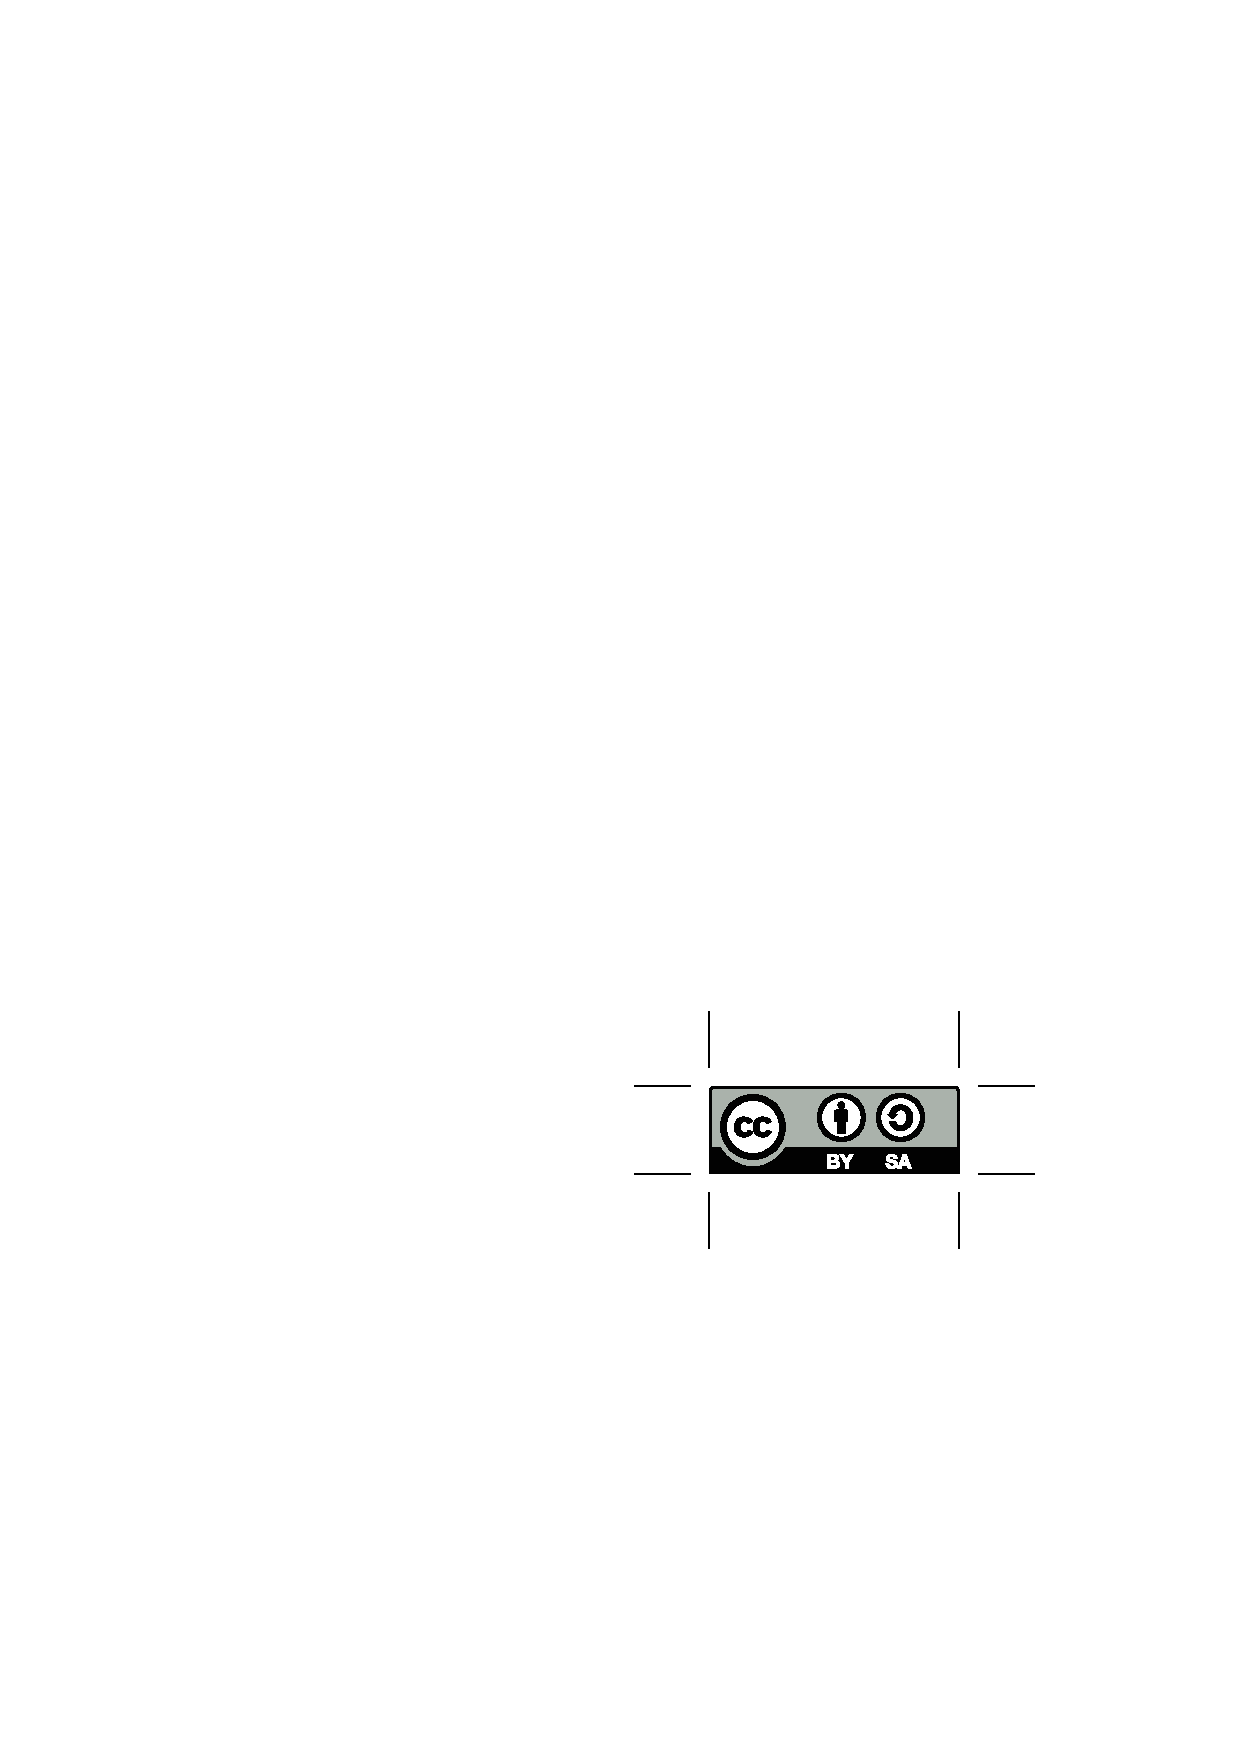
\includegraphics{by-sa}
		\\
		Published under Creative Commons Attribution-ShareAlike 4.0 International license
		\\
		https://creativecommons.org/licenses/by-sa/4.0/
	\end{center}
	\tableofcontents
	\newpage
	
	\section{The Basics}
		\subsection{Organized Code}
			\subsubsection{Indenting}
				\paragraph{}
					Indent your code with tabs if possible. Most IDEs and editors use tabs as the default. If your IDE doesn't use tabs, try and enable them in your IDE settings. Some older IDEs such as Dr. Java do not have this option. Because of this, no marks will be deducted for using spaces instead of tabs. Just make sure that your indentation is consistent.
				\paragraph{}
					There is no rule for how many characters wide indentation should be. However, most programmers use either four or eight character wide indentation. Virtually all IDEs (including Dr. Java, which uses two spaces as its default) allow this to be changed. It does not matter how wide your indentation is, as long as it is something sensible (at least two characters wide and no more than eight characters wide). The most important thing is to \textbf{be consistent}.
			\subsubsection{Whitespace}
				\paragraph{}
					Generally, some whitespace is good, but too much whitespace is bad.
				\paragraph{}
					You should have an extra line:
					\begin{itemize}
						\item After field declarations.
						\item Before a new method.
						\item Between sections of code (put a line between your local variable declarations and the processing for example), although this is more of a guideline than a rule. Use your common sense!
					\end{itemize}
				\paragraph{}
					Spaces have more complicated rules than new lines, but there are not many rules to them. For example: have a space after commas and before and after braces (unless the brace is the last character on the line). For more details on spacing, see the exemplar below.
			\subsubsection{Comments}
				\paragraph{}
					Contrary to popular belief, you do \textbf{not} need to comment every other line of your code.
				\paragraph{}
					If you are using unfamiliar libraries, it may help to use more comments, but generally, lots of comments are not needed. There is nothing wrong with having extra comments, but they are rarely necessary. If you think that your code does not make any sense without comments, you should think if it can be written in a simpler way. If it cannot, then write some comments, but you will find that you can usually make your code a lot more KISS.
				\paragraph{}
					Again, this is a guideline, not a rule, but if you feel that you need comments \textbf{beyond} the Javadoc comments, then your code might not be KISS.
	\newpage
	\section{Javadoc}
		\paragraph{}
			Proper Javadoc style consists of Javadoc comments for all fields, classes, and methods.
		\paragraph{}
			Javadoc comments are designated with two asterisks after the slash. They go on top of the method, field, or class declaration that they are explaining.
		\begin{lstlisting}[style=javasnippet]
			/** This is a Javadoc comment for a field. */
			private int commentMe;
		\end{lstlisting}
		\begin{lstlisting}[style=javasnippet]
			/**
			 * This is a Javadoc comment for a method.
			 *
			 * @param num The number to square.
			 * @return The square of the number.
			 */
			private int square(int num) {
				return num * num;
			}
		\end{lstlisting}
		\begin{lstlisting}[style=javasnippet]
			/**
			 * This is a Javadoc comment for a class.
			 * 
			 * <h2>Course Info:</h2>
			 * ICS4U0 with Krasteva, V.
			 * 
			 * @version 17.02.24
			 * @author Vincent Macri
			 */
			public class MyClass {
				// Code
			}
		\end{lstlisting}
		\paragraph{}
			This allows the Javadoc generator to generate a webpage that explains everything easily. Modern IDEs will also pick up on your Javadoc comments, and remind you what the method, field, or class does when you hover your mouse over it.
		\paragraph{}
			There is one exception to the have a Javadoc comment for every method rule. If a method is overriding another method, and your changes are small enough that the Javadoc in the parent class still makes sense, you do not need a Javadoc comment. You should, however, use the @Override notation, to explicitly state that the method is being overridden. We do this because it does not make sense to write a comment for something that is already explained well in the parent class.
		\begin{lstlisting}[style=javasnippet]
			@Override
			public void overriddenMethod() {
				// Trivial code
			}
		\end{lstlisting}
	\newpage
	\section{Exemplar}
		\lstinputlisting[language=Java]{FizzBuzzExample.java}
\end{document}
